\documentclass{report}

\usepackage[left=3cm,right=3cm,top=1cm,bottom=2cm]{geometry}
\usepackage{polski}
\usepackage[utf8]{inputenc}
\usepackage{graphicx, float}

\newenvironment{absolutelynopagebreak}
{\par\nobreak\vfil\penalty0\vfilneg
	\vtop\bgroup}
{\par\xdef\tpd{\the\prevdepth}\egroup
	\prevdepth=\tpd}

\title{%
	System pisania testów na platformie Android \\
	\large Raport inżynierski}

\author{
	Filip Malinowski\\
	\texttt{filip.malinowski@student.pwr.edu.pl}
	\and
	pod przewodnictwem Promotora dr Witolda Paluszyńskiego\\
	\texttt{witold.paluszynski@pwr.edu.pl}
}
\date{}

\begin{document}

%\maketitle

%\tableofcontents

	\chapter{Wstęp}

	Tematem pracy jest stworzenie systemu na platformę Android umożliwiającego pisanie testów na wykładach akademickich i zautomatyzowane przetworzenie wyników testów. W skład systemu wchodzą: aplikacja na system Android oraz aplikacja serwerowa, z którą aplikacja połączy się wysyłając wybrane przez użytkownika odpowiedzi.\\
	
	\chapter{Analiza problemu}
	
	Na rynku istnieją już aplikacje częściowo odpowiadające tematowi pracy inżynierskiej. Ich funkcjonalność spełnia pewne aspekty jakimi są: wybór odpowiedzi, przesyłanie odpowiedzi do serwera oraz pobieranie treści z serwera na aplikację. Najlepszym przykładem jest aplikacja nazywająca się Quizowanie\footnote{https://play.google.com/store/apps/details?id=se.feomedia.quizkampen.pl.lite}. Aplikacja ta pozwala na pobieranie i wyświetlenie pytań z serwera, wyświetlenie możliwych odpowiedzi jako przycisków dla użytkownika oraz wysłanie odpowiedzi do serwera i zweryfikowanie ich. Jej kod źródłowy jest jednak zamknięty co sprawia, że aplikacja ta jest nieprzydatna  przy tworzeniu systemu będącego tematem tej pracy.
	
	Inne aplikacje, które można wymienić to English Grammar Test\footnote{https://play.google.com/store/apps/details?id=english.grammar.test.app} lub też sameQuizy\footnote{https://play.google.com/store/apps/details?id=pl.filing.samequizy}. Ich wartość ogranicza się jednak do rozwiązań dotyczących wyglądu interfejsu aplikacji. Nie ma możliwości w legalny sposób uzyskać kodu źródłowego lub opisów rozwiązań w tych aplikacjach z racji ich komercyjnego zastosowania.
	\\
	W przypadku aplikacji serwerowej jest wiele możliwych technologii, które można zastosować przy jej tworzeniu. Możliwe protokoły jakie można użyć między aplikacją Android, a serwerem to np. TCP, UDP, POP, SMTP, HTTP czy FTP.
	
	Aplikacje serwerowe jakie można wykorzystać do obsługi zapytań aplikacji mobilnych to: Apache\footnote{https://httpd.apache.org/}, nginx\footnote{https://www.nginx.com/}, lighttpd, OpenLiteSpeed. Każdy z serwerów obsługuje FastCGI pozwalające na napisanie programu przyjmującego i przetwarzającego przychodzące zapytania. Serwery te jednak różnią się między sobą wydajnością obsługiwania zapytań. Na podstawie Linux Web Server Performance Benchmark\footnote{https://www.rootusers.com/linux-web-server-performance-benchmark-2016-results/} z 2016 można stwierdzić, że nginx oferuje największą szybkość obsługiwania zapytań.
	
	\begin{center}
		\begin{figure}[ht]
			\centering
			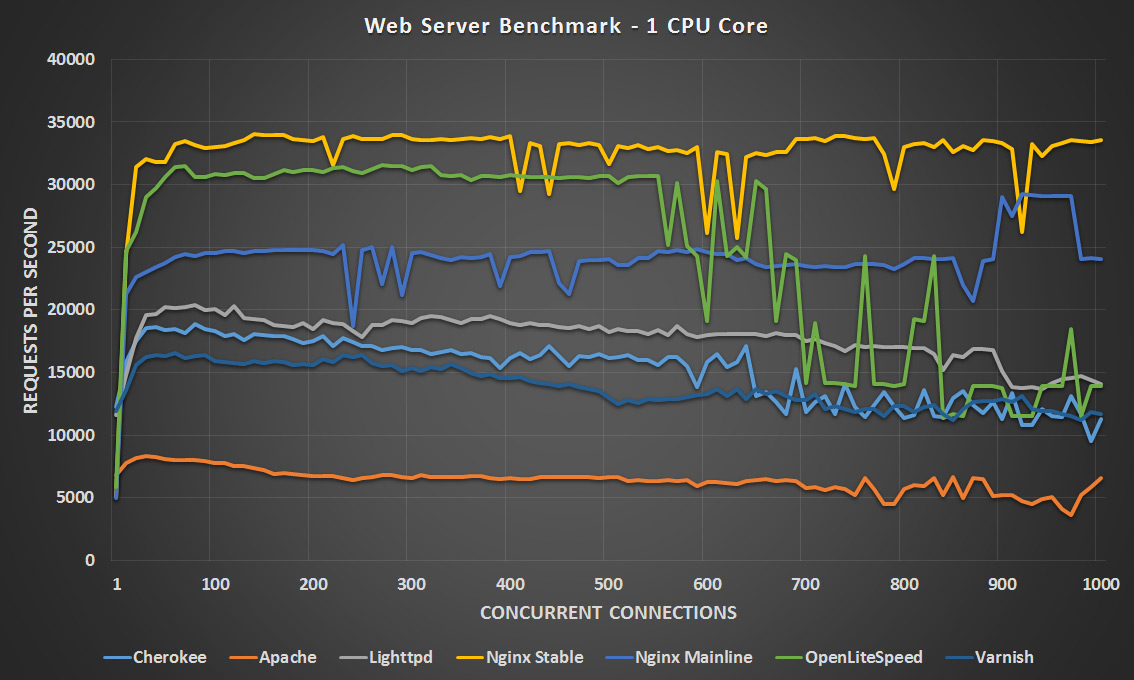
\includegraphics[scale=0.3]{web-server-performance-benchmark-1-cpu-core-1.jpg}
			\caption{Ilość obsługiwanych zapytań przy danej ilości otwartych połączeń. Źródło: Linux Web Server Performance Benchmark}
		\end{figure}
	\end{center}

	\begin{center}
		\begin{figure}[ht]
			\centering
			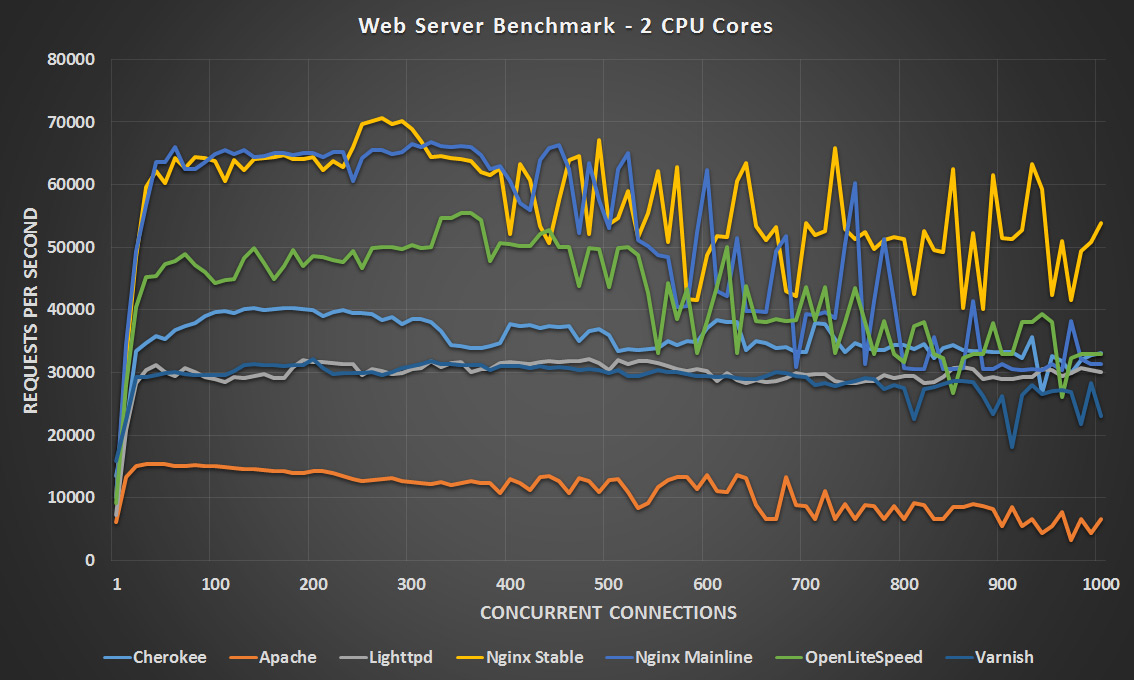
\includegraphics[scale=0.3]{web-server-performance-benchmark-2-cpu-cores-2.jpg}
			\caption{Ilość obsługiwanych zapytań przy danej ilości otwartych połączeń. Źródło: Linux Web Server Performance Benchmark}
		\end{figure}
	\end{center}
	
	Środowiska, w jakich można tworzyć aplikacje mobilne to Android Studio\footnote{https://developer.android.com/studio/index.html} oraz Qt\footnote{https://www.qt.io/}. Oba środowiska oferują duże wsparcie ze strony społeczności programistycznej oraz szeroki zestaw narzędzi. Oba pozwalają na tworzenie interfejsu użytkownika w XML oraz udostępniają klasy obiektów przydatne do wizualizowania i przetwarzania danych. Android Studio jest jednak najbardziej popularny oraz posiada najszerszą gamę narzędzi. Pozwala na dołączanie bibliotek z repozytoriów Git lub też bibliotek za pomocą wbudowanego narzędzia Maven\footnote{https://maven.apache.org/}, bieżące sprawdzanie kompatybilności użytych bibliotek z wersjami systemu Android, na które aplikacja powstaje oraz tworzenie maszyn wirtualnych do testowania napisanych aplikacji bez użycia telefonu.
	
	\chapter{Implementacja}
	
	% tutaj należy to zredagować na nowo
	
	Biorąc pod uwagę przeprowadzoną analizę problemu zdecydowano, że system do rozwiązywania testów musi być napisany od podstaw. Nie znaleziono przykładów otwartych systemów na tyle użytecznych, żeby można było użyć ich przy tworzeniu systemu. Systemy takie jak Quizowanie mają zamknięty kod i można się nimi sugerować jedynie w kwestii tworzenia interfejsu użytkownika.
	
	W trakcie pracy nad systemem do rozwiązywania testów wymagania co do tego systemu zostały doprecyzowane. Aplikacja mobilna musi być przyjazna dla użytkownika i intuicyjna. Użytkownik dalej ma możliwość pisania testów na papierze dlatego forma elektroniczna musi być wystarczająco zachęcająca. Ponadto musi też być niezawodna. Nie powinna tracić przetwarzanych w niej istotnych informacji lub wyłączać się w trakcie rozpoczęcia pisania testu. Aplikacja musi się też w niezawodny sposób łączyć z serwerem w celu przesłania odpowiedzi użytkownika lub też pozwolić na ponowne ich wysłanie po utracie połączenia. Kopie zapasowe testów muszą też być zapisywane w pamięci wewnętrznej telefonu, a ich zawartość zaszyfrowana chroniąc wrażliwe dane przed ingerencją osób nieupoważnionych. Aplikacja powinna też być weryfikowalna przez serwer, żeby nie dopuścić do wysyłania odpowiedzi z aplikacji zmodyfikowanych przez osoby trzecie. Musi też informować użytkownika odpowiednimi komunikatami wyświetlanymi na ekranie o zaistniałych problemach na każdym etapie użytkowania, żeby użytkownik wiedział w jaki sposób reagować na nieprzewidziane sytuacje.
	
	Aplikacja serwerowa musi być w stanie obsługiwać wysoki ruch, w którym przybywa średnio 10 zapytań na sekundę, dochodząc nawet do 100 na sekundę przy 100 osobowej grupie użytkowników piszących test. Docelowo powinna jednak być w stanie obsłużyć nawet 300-400 użytkowników, żeby można było ją zastosować w każdej możliwej grupie studentów na Politechnice Wrocławskiej. Serwer musi też być w stanie weryfikować aplikacje mobilne, tak aby nie przesyłać wrażliwych informacji niebezpiecznych aplikacji mobilnych. Jego struktura musi być możliwie prosta, żeby przyszłe modyfikacje były mało uciążliwe dla zarządcy całego systemu.
	
	Do komunikacji między aplikacją mobilną, a serwerem wybrany został protokół HTTP dlatego, że sieć WiFi na Politechnice Wrocławskiej ma odblokowaną komunikację na portach 80 oraz 8080. Prawdopodobnie na tych wymienionych portach sprawdzane są również użyte protokoły i ich zgodność z HTTP. Innego rodzaju protokół wykluczyłby użycie systemu w połączeniu z niezabezpieczoną politechniczną siecią WiFi co znacząco ograniczyłoby jego zastosowanie.
	
	Aplikacja mobilna przechowuje dane użytkownika takie jak: imię, nazwisko, numer indeksu oraz nazwa kursu na którym wykonywany jest test. Umożliwia też zmianę adresu serwera, na który przysyłane są odpowiedzi z testu. W menu głównym pozwala na wprowadzenie rzędu i miejsca, na którym użytkownik siedzi podczas testu, wektora wag służącego do obliczania grupy oraz ID testu jaki jest przeprowadzany. Zostało też zaimplementowane udogodnienie dla użytkownika w postaci skanera kodów QR umożliwiającego zautomatyzowane wczytanie wektora wag, ID testu i wyliczenie grupy użytkownika. Do skanowania kodów QR została wykorzystana biblioteka zxing\footnote{https://github.com/zxing/zxing} (Zebra Crossing). Po przejściu do testu wyświetlany jest ekran konfiguracyjny aplikacji gdzie użytkownik jest informowany o operacjach przeprowadzanych przed rozpoczęciem testu. Aplikacja sprawdza osiągalność serwera, do którego wysyła odpowiedzi oraz pobiera plik konfiguracyjny zawierający takie dane jak: minimalna i maksymalna wersja aplikacji dopuszczona do testu oraz klucz do szyfrowania danych w plikach testu przechowywanych na telefonie użytkownika. Po przejściu etapu konfiguracji wyświetlana jest zakładka pytania, a na niej: nr grupy w jakiej użytkownik się znajduje, nr pytania, przyciski: tak, nie, nie wiem do wysłania odpowiedzi, przyciski do dodawania pytań oraz do podsumowania testu i unikalny identyfikator sesji wygenerowany dla aktualnej sesji testowej otwartej na telefonie. Dodanie pytania wymusza przejście do następnego pytania, a UI użytkownika pozwala na przesuwanie ekranu w celu wyświetlenia innych pytań. Podsumowanie testu wyświetla ilość poprawnie przesłanych odpowiedzi "tak", "nie" oraz "nie wiem" do serwera, oraz ilość odpowiedzi zapisanych w pliku testowym. W razie różnicy w odpowiedziach przesłanych do serwera, a zapisanych w pliku aplikacja wyświetla odpowiednie ostrzeżenie sugerujące użytkownikowi powrót do testu i ponowne przesłanie odpowiedzi. Na ekranie podsumowania wyświetlany jest przycisk pozwalający powrót do testu oraz przycisk kończący test powodujący powrót do menu głównego aplikacji.
	
	Serwerem do obsługi zapytań sieciowych jest Apache. Do przetwarzania danych wykorzystano skrypt napisany w języku AWK. Skanuje on logi serwera Apache w poszukiwaniu zarejestrowanych zapytań przysłanych z aplikacji mobilnych i umożliwia zapisanie ich w formacie użytecznym dla zarządcy systemu.
	
	Napisany został też deszyfrator plików przechowywanych na telefonach użytkowników pozwalający na odzyskanie odpowiedzi w razie różnic występujących w ilości odpowiedzi wysłanych do serwera, a ilości odpowiedzi zapisanych lokalnie na telefonie.
	
	Do tworzenia plików konfiguracyjnych napisany został konfigurator. Tworzy on dokument XML zawierający klucz szyfrowania i zakres dopuszczalnych wersji aplikacji. Tworzy też plik przechowujący klucz deszyfrowania wykorzystywany w deszyfratorze.
	
	\section{Elementy aplikacji}
	
		\subsection{Widoki aplikacji}
		
		Wygląd aplikacji stanowi ważny element aplikacji. W początkowych fazach projektu rozmieszczenie elementów na ekranie telefonu komórkowego jak też ich estetyka wielokrotnie była zmieniana. Potrzebne było wypracowanie przejrzystego oraz przyjaznego dla studenta interfejsu aplikacji. W trakcie tworzenia aplikacji zauważono, że istotnym elementem jest zachowanie kompatybilności z różnymi wersjami systemu Android realizując jednolite i przewidywalne zachowanie się interfejsu.
		Na przykład nie można było zastosować kolorowania przycisków korzystając z metody setColorFilter obecnej we wszystkich wersjach systemu od Android 4.0 do Android 7.0. Efekt wywołania tej metody w systemach Android 4.0 do 4.4 był inny od efektu uzyskiwanego w systemach Android 5.0 i wyższych. Powodowało to brak kompatybilności pomiędzy tymi wersjami.\\
		
		Widoki jakie zostały zaimplementowane w aplikacji to:
		\begin{itemize}
			\item Widok główny\\
			Za jego pomocą użytkownik może wprowadzić swoje miejsce i rząd w jakim się znajduje, wektor wag służący do wyliczenia grupy na teście oraz kod testu. Na tym widoku można uruchomić również skaner kodów QR do automatycznego pobrania wektora wag i kodu testu oraz wyliczenia grupy na teście. Trzy dolne przyciski służą do wyjścia z aplikacji, ręcznego wyliczenia numeru grupy oraz przejścia do testu. Z tego widoku można również otworzyć menu, z którego można dostać się do widoku ustawień i widoku informacji.
			
			\item Widok ustawień\\
			Tutaj użytkownik może wprowadzić i zapisać w aplikacji swoje dane takie jak: imię, nazwisko, numer indeksu oraz nazwa przedmiotu. Opcjonalnie może wprowadzić inny adres serwera, na który aplikacja będzie przesyłać odpowiedzi użytkownika.
			
			\item Widok informacji\\
			W tym widoku użytkownik może się dowiedzieć z jakiej wersji aplikacji korzysta.
			
			\item Widok konfigurowania testu\\
			Tutaj użytkownik jest informowany o przebiegu połączenia testowego z serwerem, o pobraniu pliku konfiguracyjnego, oraz o sprawdzeniu poprawności klucza szyfrowania i poprawności wersji aplikacji.
			
			\item Widok testu\\
			W tym miejscu użytkownik może wybrać odpowiedzi na pytania o danym numerze, dodać nowe karty z pytaniami lub przejść do podsumowania. Do wyboru odpowiedzi służą trzy przyciski: tak, nie, nie wiem. Po wciśnięciu tych przycisków odpowiednia informacja jest zapisywana do pliku i wysyłana do serwera.
			
			\item Widok podsumowania\\
			Tutaj użytkownik może odczytać ile odpowiedzi zostało poprawnie wysłanych do serwera oraz ile odpowiedzi zostało zapisanych lokalnie na telefonie. Dwa dolne przyciski umożliwiają powrót do testu celem wprowadzenia poprawek lub wyjście z testu i powrót do widoku głównego.
			
		\end{itemize}
		
		\subsection{Interaktywne elementy na widokach}
		
		\paragraph{Rozwijane listy}
		zostały utworzone w widoku ustawień i widoku głównym. W widoku ustawień po kliknięciu na pole do edycji nazwy testu otwiera się okienko z przesuwalną listą, z której można wybrać nazwę kursu. W widoku głównym taka sama wizualnie lista wyświetla propozycje ID testu wygenerowane na podstawie nazwy kursu.
		
		\paragraph{Zmiennokształtne przyciski}
		służą do sygnalizowania asynchronicznych operacji zachodzących w trakcie konfiguracji i weryfikacji aplikacji. Za podstawę służy Android Circular Progress Button\footnote{https://github.com/flavioarfaria/circular-progress-button}, który został umieszczony na widoku ustawień. Przycisk ten w aplikacji zmienia swój kolor oraz wygląd sygnalizując:
		\begin{itemize}
			\item bezczynność - niebieski pusty przycisk
			\item przetwarzanie operacji - wirujące kółko
			\item powodzenie przetwarzania operacji - zielony przycisk z checkmark
			\item niepowodzenie przetwarzania operacji - czerwony przycisk 
		\end{itemize}
		Sygnalizowanie bezczynności zostało początkowo użyte dla jednej nieaktywnej funkcji, którą była walidacja aplikacji. Zielony kolor sygnalizuje powodzenie testowego połączenia z serwerem, poprawne pobranie pliku konfiguracyjnego oraz walidację klucza szyfrowania i dopuszczalny zakres wersji aplikacji.
		Czerwony kolor sygnalizuje niepowodzenie wyżej wymienionych operacji.
		Wirujące kółko trwa tak długo jak te asynchronicznie wykonywane operacje nie zakończą swojego działania.\\
		
		tutaj będą obrazki pokazujące jak zmienia się przycisk\\
		
		\paragraph{Przyciski zmieniające kolor}
		umieszczone są na kartach z odpowiedziami w aplikacji. Sygnalizują swoimi kolorami stan przetwarzania odpowiedzi użytkownika. Biały przycisk informuje o braku wybranej do tej pory odpowiedzi. Szary przycisk sygnalizuje poprawnie zapisaną odpowiedź do pliku testowego. Niebieski przycisk sygnalizuje poprawnie wysłaną odpowiedź na serwer.
		Jeżeli operacja zapisywania do pliku się nie powiedzie to przycisk pozostaje biały.
		Jeżeli operacja wysyłania do serwera się nie powiedzie to przycisk pozostaje szary. Użytkownik wtedy wie, że jego aktualna odpowiedź przechowywana jest jedynie lokalnie.\\
		
		tutaj będą obrazki pokazujące przykładowo wybraną odpowiedź\\
		
		\subsection{Powiadomienia}
		
		Istotnym elementem aplikacji okazały się być powiadomienia pozwalające na zrozumienie użytkownikowi zdarzeń występujących w aplikacji. Dzięki wypracowaniu zestawu chmurek oraz monitów użytkownik jest informowany o powodzeniu w edycji ustawień aplikacji, błędach występujących przy konfigurowaniu testu oraz różnych innych zdarzeniach takich jak utrata połączenia z serwerem czy też brak poprawnego testu, na który użytkownik chciał wysyłać odpowiedzi.
		
		\subsection{Komunikacja internetowa}
		
		Aplikacja komunikuje się z serwerem poprzez protokół HTTP. Odpowiedzi są wysyłane na zasadzie pobierania nagłówka pliku konfiguracyjnego XML z odpowiedziami umieszczonymi w query string. Kod otrzymany po wykonaniu zapytania jest następnie interpretowany, a jego wartość decyduje o powiadomieniu użytkownika o poprawnym lub niepoprawnym wysłaniu odpowiedzi do serwera.
	
		\subsection{Szyfrowanie plików}
	
		Początkowo pliki były szyfrowane algorytmem DES z kluczem przechowywanym w aplikacji. Było to jednak rozwiązanie niebezpieczne, ponieważ klucz szyfrowania można było uzyskać po zdekompilowaniu aplikacji. Pierwszym ulepszeniem zaimplementowanym w aplikacji było zastosowanie metody "security by obscurity", gdzie klucz szyfrowania zmieniał się w trakcie działania programu. W ten sposób sprawa jego uzyskania została utrudniona. Następnie w aplikacji zaimplementowano pobieranie dokumentu XML z ustawieniami testu. W tym dokumencie znajdował się klucz szyfrowania wykorzystywany później w algorytmie DES. W dalszym etapie wykorzystano szyfrowanie algorytmem RSA, którym zastąpiono algorytm DES, a klucz w dokumencie XML został zamieniony na 4096 bitowy klucz publiczny algorytmu RSA.
	
		\subsection{Skaner QR}
		
		W aplikacji wykorzystano również skaner kodów QR. Jak wcześniej o tym wspomniano, wykorzystano do tego bibliotekę zxing. Pozwala ona nie tylko na skanowanie kodów QR ale również kodów kreskowych, kodów Aztec i innych. Skaner skanuje kod QR wyświetlany na ekranie przez rzutnik automatyczne zapisując w aplikacji kodu testu i wektor wag. Po operacji skanowania wymusza wyliczenie nowego numeru grupy. Ułatwia to pracę z aplikacją potencjalnemu użytkownikowi oraz pozwala na zmniejszenie prawdopodobieństwa popełnienia błędu przez użytkownika przy wyliczaniu grupy na teście.
		
		\subsection{Baza danych}
		
		Do długotrwałego przechowywania danych w aplikacji wykorzystano bazę danych MySQL. W tym celu stworzono klasę imitującą bazę danych MySQL oraz klasę imitującą interfejs dostępowy do tej klasy. Interfejs został następnie wykorzystany do zapisywania informacji zawartych w widoku ustawień. Służy dodatkowo jako narzędzie do rozprowadzania informacji po innych widokach aplikacji.
		
		\subsection{Odrzucanie połączeń w trakcie testu}
		
		W trakcie testowania aplikacji na grupie studentów pojawiła się potrzeba automatycznego odrzucania przychodzących połączeń telefonicznych. W tym celu stworzono klasę na bazie wbudowanej BroadcastReceiver, która to odrzuca wszystkie przychodzące połączenia jeśli użytkownik jest w trakcie pisania testu.
		
	\section{Programy dodatkowe}
		
		\subsection{Generator konfiguracji}
		
		Generator został napisany w języku Java w wersji pozwalającej uruchomienie go tylko w linii poleceń. W parametrach wywołania tego programu podaje się kod testu, minimalną wersję aplikacji oraz maksymalną wersję aplikacji dopuszczoną do testu. Program generuje dwa pliki. Pierwszy jest dokumentem XML zawierającym klucz publiczny RSA plus dodatkowe parametry testu przeznaczone dla aplikacji Android. Drugi plik zawiera klucz prywatny RSA służący do rozszyfrowywania odpowiedzi zaszyfrowanych wcześniej kluczem publicznym.
		
		\subsection{Deszyfrator}
		
		Deszyfrator również został napisany w języku Java i umożliwia uruchomienie jedynie w linii poleceń. Początkowa wersja deszyfratora korzystała z algorytmu DES, najpierw ze stałym kluczem zapisanym w aplikacji, potem z kluczem odczytywanym z pliku. Ostatecznie stosuje algorytm RSA, a klucz prywatny pobiera z pliku.
		

	\chapter{Testowanie systemu}
	
	System został pomyślnie wykorzystany na Wydziale Mechanicznym, Automatyce i Robotyce na kursie Systemy Czasu Rzeczywistego i Sieci Komputerowe. Średnio z aplikacji korzystało około 90 osób na każdym z siedmiu wykonanych testów. Ponadto aplikacja została wykorzystana na testach na Wydziale Elektroniki, Automatyce i Robotyce na kursie SCR Systemy Operacyjne.
		
			
\end{document}